\begin{savequote}[45mm]
\ascii{Any fool can write code that a computer can understand. Good programmers write code that humans can understand.}
\qauthor{\ascii{- Martin Flower}}
\end{savequote}

\chapter{隐式树} 
\label{ch:implicit-tree}

\begin{content}

本章重点讨论批量的用例组织和用例运行的实现方式。通过引入隐式的\emph{树结构},提供了一种处理相似逻辑的一般性方法,极大地简化了客户组织用例与运行用例的实现逻辑。最后,为了区分每个测试用例,为其增加命名机制。

\end{content}

\section{测试套件}

\begin{content}

如果每个用例都需要手动地执行\ascii{run},显得极其笨拙。可以将一堆测试用例打包,用一个简单的\ascii{for}循环依次执行每个用例。

\subsection{什袭以藏}

新建一个失败的测试用例,用于打包普通的\ascii{TestCase}实例。为了确定有多少个\ascii{TestCase}被执行,可以定制一个计数器\ascii{num}。当执行完之后,断言已运行用例的数目是否符合预期。

\begin{nodiff}{test/mars/core/TestSuiteSpec.cc}
 \begin{c++}
#include <mars/core/TestSuite.h>
#include <mars/core/TestCase.h>
#include <gtest/gtest.h>

namespace {
  int num = 0;

  struct FooTest : TestCase {
  private:
    void runTest() override {
      num++;
    }
  };
}

TEST(TestSuite, pack_multi_test_cases_into_test_suite) {
  TestSuite suite;
  suite.add(new FooTest);
  suite.add(new FooTest);

  suite.run();

  ASSERT_EQ(2, num);
}
 \end{c++}
\end{nodiff}

\subsubsection{通过编译}

为了快速通过编译,创建\ascii{TestSuite}的头文件。其中,\ascii{TestSuite}仅对\ascii{TestCase}的指针类型产生依赖,前置声明\ascii{struct TestCase}即可。此外,为了快速通过编译,不必提前设计私有的数据结构。

\begin{nodiff}{include/mars/core/TestSuite.h}
 \begin{c++}
struct TestCase;

struct TestSuite {
  void add(TestCase* test);
  void run();
};
 \end{c++}
\end{nodiff}

\begin{episode}{最小化编译时依赖: 前置声明 VS. 包含头文件}

\begin{content}

当头文件中仅对类的声明产生依赖,那么前置声明是一种有效降低编译时依赖的重要技术。相反,头文件包含了本不应该包含的头文件,其编译时依赖将被间接污染到其他文件中,重编译将成为大概率事件。

\subsubsection{前置声明}

在包含头文件还是前置声明抉择中,其依据的规则非常简单。在如下场景前置声明即可,无需包含头文件。

\begin{enum}
  \eitem{\ascii{指针}}
  \eitem{\ascii{引用}}
  \eitem{\ascii{返回值}}
  \eitem{\ascii{函数参数}}
\end{enum}

\subsubsection{包含头文件}

但是,如果编译器需要知道实体的确切内容,包括类的大小、布局、值等强编译时依赖信息,则必须包含头文件。强编译时依赖包括如下几种场景。

\begin{enum}
  \eitem{\ascii{继承}}
  \eitem{\ascii{宏}}
  \eitem{\code{inline}}
  \eitem{\code{template}}
  \eitem{\ascii{引用类内部成员时}}
  \eitem{\ascii{值类型的类成员变量}}  
  \eitem{执行\code{sizeof}运算}  
  \eitem{\code{typedef/using}类型别名}
\end{enum}

\subsubsection{样例}

以验证\ascii{TestCase.h}的自满足性为例。从上到下,从左到右,模拟编译期的行为判定编译时依赖的名字。因为继承于\ascii{TestFixture, Test},继承是一种编译时强依赖,必须包含相应的头文件。

接着,其构造函数依赖于\code{std::string},它来自标准库\footnote{\code{std::string}并非普通的类,它实际是\code{basci\_string}的一个别名:\code{using string = basic\_string<char>;} 一般地,当依赖于标准库的名字,基本需要包含头文件,而非前置声明。},本来需要包含\ascii{std::string}的头文件。但是,考虑到覆写的\ascii{getName}返回值也依赖于\code{std:string}。可以推断,\ascii{TestCase}的某个基类肯定已经包含了\code{std::string}的头文件;否则,该基类的头文件不能自满足,需要优先处理。

最后,再此分析\ascii{TestResult}的依赖关系,本来需要前置声明\ascii{TestResult}。但是,\ascii{run}成员函数也被覆写了。可以推断,\ascii{TestCase}的某个基类肯定已经前置声明\ascii{TestResult}了,\ascii{TestCase}就不用再多此一举,再重复声明一次了。

如上分析,\ascii{TestCase.h}只需包含\ascii{Test.h, TestFixture.h}的头文件,便能够自满足了。

\begin{c++}[title={\ttfamily{验证头文件的自满足性: include/mars/core/TestCase.h}}]
#include <mars/core/Test.h>
#include <mars/core/TestFixture.h>

struct TestCase : private TestFixture, Test {
  explicit TestCase(const std::string &name="");
    
private:
  void run(TestResult &result) override;
  std::string getName() const override;

private:
  virtual void runTest() {}
    
private:
  const std::string name;
};
\end{c++}

\end{content}
\end{episode}

\subsubsection{通过测试}

在\ascii{TestSuite.h}中设计最简单的私有数据结构。因为\ascii{TestSuite}强依赖于\ascii{std::vector}的值类型,因此需要包含头文件\ascii{#include <vector>}。在实现文件中,可以快速显式实现\ascii{TestSuite::run}的逻辑。

\begin{diff}{src/mars/core/TestSuite.cc}
 \begin{minicpp}
#include <vector>

struct TestCase;

struct TestSuite {
  void add(TestCase* test);
  void run();

private:
  std::vector<TestCase*> tests;
};
 \end{minicpp}
\tcblower
 \begin{minicpp}
#include <mars/core/TestSuite.h>
#include <mars/core/TestCase.h>

void TestSuite::add(TestCase* test) {
  tests.push_back(test);
}

void TestSuite::run() {
  for (auto test : tests) {
    test->run();
  }
}
 \end{minicpp}
\end{diff}

\begin{episode}{验证头文件的自满足性}
\begin{content}

所谓头文件自满足性,即头文件自身是可编译成功的。为了验证头文件的自满足性,其实现文件需要第一个包含对应的头文件。如果此头文件不自满足,自然会导致编译失败,此方法是验证头文件是否自满足的一个有效方法。

\subsubsection{样例}

例如,对于头文件\ascii{TestSuite.h},在其相应的\ascii{TestSuite.cc}之中,需要第一个包含自己的头文件。

\begin{inlinediff}
 \begin{minicpp}
// 反例
#include <mars/core/TestCase.h>
#include <mars/core/TestSuite.h>
 \end{minicpp} 
\tcblower
 \begin{minicpp}
// 正例
#include <mars/core/TestSuite.h>
#include <mars/core/TestCase.h>
 \end{minicpp} 
\end{inlinediff}

头文件作为代码所有者对外公开\ascii{API}的重要途径。在发布之前,有责任保证其可用性,及其最小依赖性。如果一个头文件不自满足,当客户需要引用该头文件时,则需要客户自行承担寻找相关依赖的职责。客户因缺乏相关上下文信息,寻找缺失的依赖并非易事。

\subsubsection{特例:泛型、内联、宏定义}

在极端条件下,头文件可能不存在相应的实现文件。例如,模板类或模板函数,内联函数,宏定义。此时,可以创建相应的测试文件,第一个包含其对应的头文件,校验头文件的自满足性;并对该模板实例化,实施简单的测试,确保编译与功能正确。

\begin{c++}[title={\ttfamily{实现ScopedExit:include/mars/util/ScopedExit.h}}]
#include <mars/util/Symbol.h>

template <typename F>
struct ScopedExit {
  ScopedExit(F f) : f(f) {
  }

  ~ScopedExit() { 
    f(); 
  }

private:
  F f;
};

template <typename F>
ScopedExit<F> make_scoped_exit(F f) {
  return ScopedExit<F>(f);
};

#define SCOPED_EXIT(f) auto UNIQUE_NAME(scoped_exit_) = make_scoped_exit(f)
\end{c++}

其中,\ascii{UNIQUE\_NAME}是一个通用的宏,将其放在基础设施之中。

\begin{c++}[title={\ttfamily{实用宏:include/mars/util/Symbol.h}}]
#define __DO_JOIN_AGAIN(symbol1, symbol2) symbol1##symbol2
#define __DO_JOIN(symbol1, symbol2) __DO_JOIN_AGAIN(symbol1, symbol2)

#define JOIN(symbol1, symbol2) __DO_JOIN(symbol1, symbol2)
#define UNIQUE_NAME(prefix) JOIN(prefix, __COUNTER__)
\end{c++}

在测试文件中,第一个包含该头文件,并尝试最简单的单元测试。

\begin{c++}[title={\ttfamily{测试ScopedExit:test/mars/util/ScopedExitSpec.cc}}]
#include <mars/util/ScopedExit.h>
#include <gtest/gtest.h>

TEST(ScopedExitSpec, delete_memeory_safely) {
  auto p = new int;
  SCOPED_EXIT([p] {
    delete p;
  });
}
\end{c++}

\end{content}
\end{episode}

\subsection{内存泄露}

\ascii{TestSuite}持有若干动态分配的\ascii{TestCase}实例,引入析构函数释放动态内存。\ascii{Google Test}貌似没有提供内存泄露的检查机制,需要依赖于程序员的既有经验和自我判断。

\begin{diff}{include/mars/core/TestSuite.h}
 \begin{minicpp}
#include <vector>

struct TestCase;

struct TestSuite {
  ~TestSuite();

  void add(TestCase* test);
  void run();

private:
  std::vector<TestCase*> tests;
}; \end{minicpp}
\tcblower
 \begin{minicpp}
#include "mars/core/TestSuite.h"
#include "mars/core/TestCase.h"

void TestSuite::add(TestCase* test) {
  tests.push_back(test);
}

TestSuite::~TestSuite() {
  for (auto test : tests) {
    delete test;
  }
}

void TestSuite::run() {
  for (auto test : tests) {
    test->run();
  }
}
 \end{minicpp}
\end{diff}

\subsection{消除重复}

为了消除析构函数与\ascii{run}之间的重复设计,提取一个公共的\ascii{foreach}泛型函数。注意,不要在头文件直接实现该模板函数,最小化编译时的依赖。

\begin{diff}{include/mars/core/TestSuite.h}
 \begin{minicpp}
#include <vector>

struct TestCase;

struct TestSuite {
  ~TestSuite();

  void add(TestCase* test);
  void run();

private:
  std::vector<TestCase*> tests;
};
 \end{minicpp}
\tcblower
 \begin{minicpp}
#include <vector>

struct TestCase;

struct TestSuite {
  ~TestSuite();

  void add(TestCase* test);
  void run();

private:
  template <typename F>
  void foreach(F f) const;

private:
  std::vector<TestCase*> tests;
};
 \end{minicpp}
\end{diff}

可以使用\ascii{Lambda}表达式定制各种算子,实现差异化配置,实现对迭代算法的高度复用。

\begin{diff}{src/mars/core/TestSuite.cc}
 \begin{minicpp}
#include <mars/core/TestSuite.h>
#include <mars/core/TestCase.h>

void TestSuite::add(TestCase* test) {
  tests.push_back(test);
}

TestSuite::~TestSuite() {
  for (auto test : tests) {
    delete test;
  }
}

void TestSuite::run() {
  for (auto test : tests) {
    test->run();
  }
}
 \end{minicpp}
\tcblower
 \begin{minicpp}
#include <mars/core/TestSuite.h>
#include <mars/core/TestCase.h>

void TestSuite::add(TestCase* test) {
  tests.push_back(test);
}

template <typename F>
inline void TestSuite::foreach(F f) const {
  for (auto test : tests) {
    f(test);
  }
}

TestSuite::~TestSuite() {
  foreach([](auto test) {
    delete test;
  });
}

void TestSuite::run() {
  foreach([](auto test) {
    test->run();
  });
}
 \end{minicpp}
\end{diff}

设计分离了两个变化方向,使其能够独立变化。

\begin{enum}
  \eitem{\ascii{迭代算法:因存储结构变化而变化(目前实现为线性表);}}
  \eitem{\ascii{处理算子:存在删除,计数,运行等操作。}}
\end{enum}

\subsubsection{弃用std::for\_each}

此处未使用\ascii{std::for\_each},即使使用\ascii{std::for\_each},也存在重复逻辑,代码为证。

\begin{nodiff}{src/mars/core/TestSuite.cc}
 \begin{c++}
#include <mars/core/TestSuite.h>
#include <mars/core/TestCase.h>
#include <algorithm>

TestSuite::~TestSuite() {
  std::for_each(tests.begin(), test.end(), [](auto test){
    delete test;
  });
}

void TestSuite::run() {
  std::for_each(tests.begin(), test.end(), [](auto test){
    test->run();
  });
}
 \end{c++}
\end{nodiff}

为了彻底消除重复,避免重复两次\ascii{begin, end}的调用逻辑,提取了公共的成员函数\ascii{TestSuite::foreach}。

\begin{nodiff}{src/mars/core/TestSuite.cc}
 \begin{c++}
#include <mars/core/TestSuite.h>
#include <mars/core/TestCase.h>
#include <algorithm>

template <typename F>
void TestSuite::foreach(F f) const {
  std::for_each(tests.begin(), test.end(), f);
}

TestSuite::~TestSuite() {
  foreach([](auto test){
    delete test;
  });
}

void TestSuite::run() {
  foreach([](auto test){
    test->run();
  });
}
 \end{c++}
\end{nodiff}

经过重构,两种方法殊途同归,都提取了公共的成员函数\ascii{TestSuite::foreach}。但是,依赖于\ascii{std::for\_each}实现,需要额外引入整个\code{\#include <algorithm>},有点得不偿失。而使用内置的、基于范围的\ascii{for}循环,不仅提高了代码的可读性,而且降低了编译时依赖,甚至在运行时性能略微提升。\footnote{\code{std::for\_each}返回了一元的回调函数,产生一次额外的拷贝。即使存在\ascii{RVO}机制,但却依赖于编译器的具体实现。}

\begin{diff}{src/mars/core/TestSuite.cc}
 \begin{minicpp}
#include <mars/core/TestSuite.h>
#include <mars/core/TestCase.h>
#include <algorithm>

template <typename F>
void TestSuite::foreach(F f) {
  std::for_each(tests.begin(), test.end(), f);
}

TestSuite::~TestSuite() {
  foreach([](auto test){
    delete test;
  });
}

void TestSuite::run() {
  foreach([](auto test){
    test->run();
  });
}
 \end{minicpp}
\tcblower
 \begin{minicpp}
#include <mars/core/TestSuite.h>
#include <mars/core/TestCase.h>

template <typename F>
void TestSuite::foreach(F f) {
  for (auto test : tests) {
    f(*test);
  }
}

TestSuite::~TestSuite() {
  foreach([](auto test) {
    delete test;
  });
}

void TestSuite::run() {
  foreach([](auto test){
    test->run();
  });
}
 \end{minicpp}
\end{diff}

综上述,相对于\ascii{std::for\_each}泛型算法,我更偏爱\emph{基于范围的\ascii{for}循环}。

\begin{episode}{基于范围的for语句}
\begin{content}

在\ascii{C++98}里,\ascii{foreach}的典型实现方法如下所示。不幸的是,它引入了复杂的\ascii{typedef typename}类型别名机制\footnote{\cpp{}也因诸如此类冗余的、复杂的类型说明,招致各种非议。}。

 \begin{c++}[title={\ttfamily{实现foreach:应用for循环,C++98}}]
template<typename T, typename F>
void foreach(const std::vector<T>& c, F f) {
  typedef typename std::vector<T>::const_iterator Iterator;
  for (Iterator first = c.begin(), last = c.end(); first != last; ++first) {
    f(*first);
  }
}
 \end{c++}

得益于\ascii{C++11}自动类型推演,可以去除\ascii{typedef}类型别名。

 \begin{c++}[title={\ttfamily{实现foreach:应用for循环,auto类型推演,C++11}}]
template<typename T, typename F>
void foreach(const std::vector<T>& c, F f) {
  for (auto first = c.begin(), last = c.end(); first != last; ++first) {
    f(*first);
  }
}
 \end{c++}

甚至,可以使用基于范围的\ascii{for}语句替代常规的\ascii{for}循环。

 \begin{c++}[title={\ttfamily{实现foreach:应用基于范围的\ascii{for},C++11}}]
template<typename T, typename F>
void foreach(const std::vector<T>& c, F f) {
  for (const T& e : c) {
    f(e);
  }
}
 \end{c++}

可以将\ascii{auto}类型推演机制实施到底,\ascii{foreach}实现变得更加简单、抽象和实用。

 \begin{c++}[title={\ttfamily{实现foreach:应用基于范围的\ascii{for},auto类型推演,C++11}}]
template<typename T, typename F>
void foreach(const std::vector<T>& c, F f) {
  for (const auto& e : c) {
    f(e);
  }
}
 \end{c++}

遗憾的是,\ascii{foreach}不够泛型,它只能接受\ascii{std::vector},而不能接受其他容器类型,例如\ascii{std::list, std::deque, std::set}。重构\ascii{foreach}接口,使其容器类型完全泛型化,甚至能够接受临时对象\footnote{因为容器类型使用的是\ascii{const}引用类型。}。

 \begin{c++}[title={\ttfamily{实现foreach:容器泛化,C++11}}]
template<typename Container, typename F>
void foreach(const Container& c, F f) {
  for (const auto& e : c) {
    f(e);
  }
}
 \end{c++}

\ascii{STL}标准库,进一步泛化容器访问的机制,使用迭代器的开闭区间\code{[first, last)}表示。

 \begin{c++}[title={\ttfamily{实现for\_each:STL实现}}]
template<typename Iterator, typename F>
F for_each(Iterator first, Iterator last, F f) {
  for (; first != last; ++first) {
    f(*first);
  }
  return f;
}
 \end{c++}
\end{content}
\end{episode}

\end{content}

\section{嵌套结构}

\begin{content}

为了实现更好的可扩展性,\ascii{TestSuite}不仅能打包\ascii{TestCase}实例,也应该能够打包\ascii{TestSuite}的子实例,实现隐式的树结构,如\refig{test-case-tree}所示。

\begin{figure}[H]
\centering
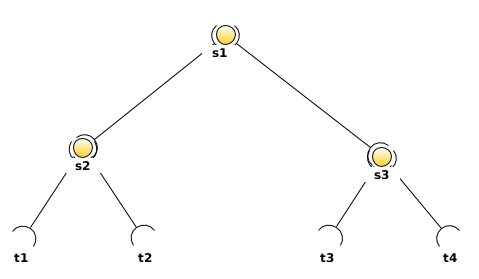
\includegraphics[width=0.8\textwidth]{figures/xunit/test-tree-example.png}
\caption{用例树:TestSuite(s1, s2, s3),TestCase(t1,t2,t3,t4)}
 \label{fig:test-case-tree}
\end{figure}

\subsection{测试依赖}

当执行用例时,确保\ascii{num}被初始化为\ascii{0};否则测试用例之间存在数据脏写的错误依赖。经过重构,\ascii{num}在\ascii{TestSuiteSpec::SetUp}时初始化为\ascii{0}值。

遗憾的是,\ascii{num}作用域依然属于匿名命名空间,而其初始化行为被搬迁至\ascii{TestSuiteSpec}的类域中。理想情况下,\ascii{num}也应搬迁至同一个类域中,并由该类的构造函数完成初始化,该重构留待后续处理。

\begin{diff}{test/mars/core/TestSuiteSpec.cc}
 \begin{minicpp}
#include <mars/core/TestSuite.h>
#include <mars/core/TestCase.h>
#include <gtest/gtest.h>

namespace {
  int num = 0;

  struct FooTest : TestCase {
  private:
    void runTest() override {
      num++;
    }
  };
}

TEST_F(TestSuiteSpec, pack_test_cases_into_test_suite) {
  TestSuite suite;
  suite.add(new FooTest);
  suite.add(new FooTest);

  run(suite);

  ASSERT_EQ(2, num);
}
 \end{minicpp}
\tcblower
 \begin{minicpp}
#include <mars/core/TestSuite.h>
#include <mars/core/TestCase.h>
#include <gtest/gtest.h>

namespace {
  int num = 0;

  struct FooTest : TestCase {
  private:
    void runTest() override {
      num++;
    }
  };

  struct TestSuiteSpec : testing::Test {
  private:
    void SetUp() override {
      num = 0;  // IMPORTANT: reset counter.
    }
  };
}

TEST_F(TestSuiteSpec, pack_test_cases_into_test_suite) {
  TestSuite suite;
  suite.add(new FooTest);
  suite.add(new FooTest);

  suite.run();

  ASSERT_EQ(2, num);
}
 \end{minicpp}
\end{diff}

\subsection{测试用例}

在既有的测试装置上,新增一个失败的测试用例。此处没有直接调用\ascii{TestSuite::run},而是使用更为抽象的\ascii{Test::run},测试装置将更加稳定。

在实现\ascii{TestSuiteSpec::run}时,显式地使用域限定符\ascii{::Test},避免与\ascii{testing::Test}产生二义性而导致编译失败。

\begin{nodiff}{test/mars/core/TestSuiteSpec.cc}
 \begin{c++}
#include <mars/core/TestSuite.h>
#include <mars/core/TestCase.h>
#include <gtest/gtest.h>

namespace {
  int num = 0;

  struct FooTest : TestCase {
  private:
    void runTest() override {
      num++;
    }
  };

  struct TestSuiteSpec : testing::Test {
  private:
    void SetUp() override {
      num = 0;  // IMPORTANT: reset counter.
    }

  protected:
    void run(::Test& test) {
      test.run();
    }
  };
}

TEST_F(TestSuiteSpec, package_sub_test_suite_into_outter_test_suite) {
  auto inner = new TestSuite;
  inner->add(new FooTest);

  TestSuite outter;
  outter.add(new FooTest);
  outter.add(inner);

  run(outter);

  ASSERT_EQ(2, num);
} 
\end{c++}
\end{nodiff}

\begin{episode}{最小化作用域}

\begin{content}

在古老的\ascii{C}程序设计语言中,要求在函数的开头实现声明所有的变量,这种代码风格和习惯被错误地保留。过早声明变量不仅使得变量作用域过早地扩展,而且会导致其过晚地终结,从而可能引入不经意的错误。例如,

 \begin{c++}[title={\ttfamily{while循环}}]
auto i = c1.iterator();
while (i.hasNext()) {
  doSomething(i.next());
}

auto i2 = c2.iterator();
while (i.hasNext()) {           // BUG!!!, should be i2.
  doSomething(i2.next());
}
 \end{c++}

当然,解决此类问题,最简单的办法就是引入代码块,将错误控制在编译时。

 \begin{c++}[title={\ttfamily{while循环}}]
{
  auto i = c1.iterator();
  while (i.hasNext()) {
    doSomething(i.next());
  }
}

{
  auto i2 = c2.iterator();
  while (i.hasNext()) {           // Compiler will be failed!
    doSomething(i2.next());
  }
}
 \end{c++}

为了缩小局部变量的作用域,可以使用\ascii{for}循环替代\ascii{while}循环,因为\ascii{for}循环提供了初始器,天然支持代码块。

 \begin{c++}[title={\ttfamily{for循环}}]
for (auto i = c1.iterator(); i.hasNext()) {
  use(i.next());
}

for (auto i = c2.iterator(); i.hasNext()) {
  use(i.next());
}
 \end{c++}

追其根因,两段代码最大的问题不是\ascii{while}与\ascii{for}之间的抉择,而是重复设计。因此,消除重复才能根除所有潜在的隐患\footnote{\ascii{Container}属于第三方集合库,并非\ascii{STL}。}。

 \begin{c++}[title={\ttfamily{for循环}}]
template <typename T>
void foreach(const Container<T>& c) {
  for (auto i = c.iterator(); i.hasNext()) {
    use(i.next());
  } 
}
 \end{c++}

遗憾的是,目前仅\ascii{for}语句提供了初始器,直至\ascii{C++17}才完备地支持了\ascii{switch, if}语句的初始器。例如,\ascii{std::set::insert}返回一个\ascii{std::pair},客户在\ascii{C++17}之前可能使用如下的代码风格。

 \begin{c++}[title={\ttfamily{插入元素:C++17之前}}]
std::set<int> nums;

auto result = nums.insert(0);
if (result->second) {
  use(*result->first);
}
 \end{c++}

如果使用\ascii{C++17},代码实现可以更加简单和安全。

 \begin{c++}[title={\ttfamily{插入元素:if初始化器与结构性绑定,C++17}}]
std::set<int> nums;

if (auto [i, succ] = nums.insert(0); succ) {
  use(*i);
}
 \end{c++}

\end{content}
\end{episode}

\subsection{提取抽象}

\ascii{TestCase}与\ascii{TestSuite}两者存在共性,但也存在差异。两者类型不兼容,导致目前用例是失败的。通过提取\ascii{TestCase}与\ascii{TestSuite}的共同抽象\ascii{Test},从而使得用例的组织更加灵活。

\begin{nodiff}{include/mars/core/Test.h}
 \begin{c++}
struct Test {
  virtual void run() = 0;
  virtual ~Test() {}
};
 \end{c++}
\end{nodiff}

\begin{episode}{抽象的接口类型}

\begin{content}

事实上,\cpp{}并没有“接口”这个术语。按照习惯,常常将只包含\ascii{pure virtual}函数的抽象类称为\emph{接口}。这是一个误区,因为\cpp{}是灵活而自由的。\cpp{}的类可以包含\ascii{pure virtual},或包含具有默认行为的\ascii{virtual}函数,或包含非\ascii{virtual}函数;也可以包含私有成员变量,或包含私有成员函数。一切皆根据具体情况,随机应变。

自由是一把双刃剑。虽然可以给设计带来了弹性,但也极大地提高了普通用户的门槛。接下来,归纳分类常见的几类抽象接口类型。

\subsubsection{函数式接口类型}

这是最简单的,也是最抽象的接口类型。它拥有一个最基本的特征,除虚析构函数之外,有且仅有一个纯虚函数。

 \begin{c++}
struct Description;

struct SelfDescribing {
  virtual ~SelfDescribing() {}
  virtual void describeTo(Description& desc) const = 0;
};
 \end{c++}

\subsubsection{纯接口类型:无成员变量}

此类接口类型,实际是函数式接口的一个超集。除虚析构函数之外,它可以拥有一个或多个纯虚函数。

 \begin{c++}
template <typename T>
struct Matcher : SelfDescribing {
  virtual bool matches(const T& actual) const = 0;
  virtual void describeMismatch(const T& actual, Description& desc) const = 0;
};
 \end{c++}

\subsubsection{扩展接口类型:无成员变量}

此类接口类型,是纯接口类型的一个超集。它不仅包含纯虚函数,也包含默认实现的虚函数。甚至,可以提取私有的成员函数。

 \begin{c++}
#include <hamcrest/core/Description.h>

template <typename T>
struct Matcher : SelfDescribing {
  virtual bool matches(const T& actual) const = 0;

  virtual void describeMismatch(const T& actual, Description& desc) const {
    desc.appendText("was ").appendValue(actual);
  }
};
 \end{c++}

\subsubsection{广义接口类型:存在成员变量}

此类接口类型,是扩展接口类型的一个超集。它可以包含任意类型的成员函数,也包含成员变量。

 \begin{c++}
#include <string>

struct TestResult;

struct Test {
  explicit Test(const std::string& name = "");
  const std::string& getName() const;

  virtual int countTestCases() const = 0;
  virtual void run(TestResult&) = 0;

  virtual ~Test() {}

private:
  std::string name;
};
 \end{c++}

\end{content}
\end{episode}

\subsubsection{重构TestCase}

重构\ascii{TestCase},所有显式声明的成员函数都是\ascii{private}。尤其关注被覆写的\ascii{TestCase::run},被显式地声明为\ascii{private},逼迫用户使用抽象接口\ascii{Test::run},而“面向接口编程”是一种良好的\ascii{OO}设计原则。

\begin{diff}{include/mars/core/TestCase.h}
 \begin{minicpp}
#include <mars/core/TestFixture.h>

struct TestCase : private TestFixture {
  void run();

private:
  virtual void runTest() {}
};
 \end{minicpp}
\tcblower
 \begin{minicpp}
#include <mars/core/Test.h>
#include <mars/core/TestFixture.h>

struct TestCase : Test, private TestFixture {
private:
  void run() override;

private:
  virtual void setUp() {}
  virtual void runTest() {}
  virtual void tearDown() {}
};
 \end{minicpp}
\end{diff}

\subsubsection{重构TestSuite}

同理,重构\ascii{TestSuite}继承于抽象类型\ascii{Test},并将所有引用\ascii{TestCase}的具体类型,替换为\ascii{Test}的抽象类型。

\begin{diff}{include/mars/core/TestSuite.h}
 \begin{minicpp}
#include <vector>

struct TestCase;

struct TestSuite {
  ~TestSuite();

  void add(TestCase* test);
  void run();

private:
  template <typename F>
  void foreach(F f) const;

private:
  std::vector<TestCase*> tests;
};
 \end{minicpp}
\tcblower
 \begin{minicpp}
#include <vector>
#include <mars/core/Test.h>

struct TestSuite : Test {
  ~TestSuite();
  void add(Test* test);

private:
  void run() override;

private:
  template <typename F>
  void foreach(F f) const;

private:
  std::vector<Test*> tests;
};
 \end{minicpp}
\end{diff}

\ascii{TestSuite}的实现也应该使用\ascii{Test}的抽象类型。幸运的是,既有代码使用\ascii{auto}的自动类型推演,实现文件仅需要修改\ascii{TestSuite::add}函数签名便可以通过测试了,充分体现了\ascii{auto}自动类型推演的优势。

\begin{diff}{src/mars/core/TestSuite.cc}
 \begin{minicpp}
#include <mars/core/TestSuite.h>
#include <mars/core/TestCase.h>

void TestSuite::add(TestCase* test) {
  tests.push_back(test);
}

template <typename F>
inline void TestSuite::foreach(F f) const {
  for (auto test : tests) {
    f(test);
  }
}

TestSuite::~TestSuite() {
  foreach([](auto test) {
    delete test;
  });
}

void TestSuite::run() {
  foreach([](auto test) {
    test->run();
  });
} 
 \end{minicpp}
\tcblower
 \begin{minicpp}
#include <mars/core/TestSuite.h>

void TestSuite::add(Test* test) {
  tests.push_back(test);
}

template <typename F>
inline void TestSuite::foreach(F f) const {
  for (auto test : tests) {
    f(test);
  }
}

TestSuite::~TestSuite() {
  foreach([](auto test) {
    delete test;
  });
}

void TestSuite::run() {
  foreach([](auto test) {
    test->run();
  });
}
 \end{minicpp}
\end{diff}

如\refig{test-tree}所示,通过\ascii{Test, TestCase, TestSuite}拼装组合,可以方便地构建复杂树形结构的用例图。至此,\ascii{xUnit Mars}的核心领域模型基本构建完毕。

\begin{figure}
\centering
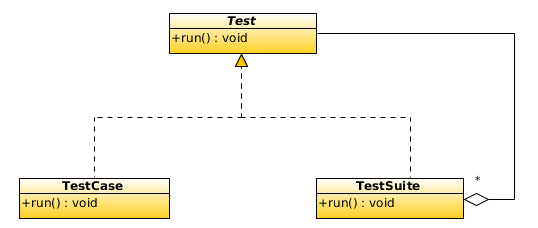
\includegraphics[width=0.8\textwidth]{figures/xunit/test-tree.png}
\caption{组合:构建隐式树}
 \label{fig:test-tree}
\end{figure}

\end{content}

\section{命名机制}

\begin{content}

可以给每个\ascii{TestCase, TestSuite}命名,方便后期用例的定位与调试。

\subsection{命名用例}

\begin{nodiff}{test/mars/core/TestCaseSpec.cc}
 \begin{c++}
#include <gtest/gtest.h>
#include <mars/core/TestCase.h>

TEST(NamedTestCase, named_test_case) {
  TestCase test("test case")
  assertName("test case", test.getName());
}
 \end{c++}
\end{nodiff}

\subsubsection{重构TestCase}

在\ascii{TestCase}中覆写\ascii{getName}成员函数。其中,为默认构造函数提供空字符串,保证既有的用例都能通过。

\begin{diff}{include/mars/core/TestCase.h}
 \begin{minicpp}
#include <mars/core/Test.h>
#include <mars/core/TestFixture.h>

struct TestCase : Test, private TestFixture {
private:
  void run() override;

private:
  virtual void runTest() {}
};
 \end{minicpp}
\tcblower
 \begin{minicpp}
#include <mars/core/Test.h>
#include <mars/core/TestFixture.h>

struct TestCase : Test, private TestFixture {
  explicit TestCase(const std::string& = "");
  const std::string& getName() const;

private:
  void run() override;

private:
  virtual void runTest() {}

private:
  std::string name;
};
 \end{minicpp}
\end{diff}

在\ascii{TestCase.cc}中实现文件中,也极为简单。

\begin{diff}{src/mars/core/TestCase.cc}
 \begin{minicpp}
#include <mars/core/TestCase.h>

void TestCase::run() {
  setUp();
  runTest();
  tearDown();
}
 \end{minicpp}
\tcblower
 \begin{minicpp}
#include <mars/core/TestCase.h>

TestCase::TestCase(const std::string& name)
  : name(name) {}

const std::string& TestCase::getName() const {
  return name;
}

void TestCase::run() {
  setUp();
  runTest();
  tearDown();
}
 \end{minicpp}
\end{diff}

测试通过。

\subsection{命名套件}

依葫芦画瓢,\ascii{TestSuite}的名字实现与\ascii{TestCase}雷同。新增一个失败的用例,驱动实现\ascii{TestSuite}的命名机制。

\begin{nodiff}{test/mars/core/TestSuiteSpec.cc}
 \begin{c++}
#include <gtest/gtest.h>
#include <mars/core/TestSuite.h>

TEST(NamedTestSuite, named_test_suite) {
  TestSuite suite("test suite")
  assertName("test suite", suite.getName());
}
 \end{c++}
\end{nodiff}

\subsubsection{重构TestSuite}

添加私有字段\ascii{name},增加携带默认参数的构造函数,及其实现\ascii{getName}成员函数。

\begin{diff}{include/mars/core/TestSuite.h}
 \begin{minicpp}
#include <vector>
#include <mars/core/Test.h>

struct TestSuite : Test {
  ~TestSuite();
  void add(Test* test);

private:
  void run() override;

private:
  template <typename F>
  void foreach(F f) const;

private:
  std::vector<Test*> tests;
};
 \end{minicpp}
\tcblower
 \begin{minicpp}
#include <vector>
#include <mars/core/Test.h>

struct TestSuite : Test {
  explicit TestSuite(const std::string& = "");
  ~TestSuite();

  const std::string& getName() const;
  void add(Test* test);

private:
  void run() override;

private:
  template <typename F>
  void foreach(F f) const;

private:
  std::string name;
  std::vector<Test*> tests;
};
 \end{minicpp}
\end{diff}

在实现文件中,实现相关成员函数。

\begin{diff}{src/mars/core/TestSuite.cc}
 \begin{minicpp}
#include <mars/core/TestSuite.h>

void TestSuite::add(Test* test) {
  tests.push_back(test);
}

template <typename F>
inline void TestSuite::foreach(F f) const {
  for (auto test : tests) {
    f(test);
  }
}

TestSuite::~TestSuite() {
  foreach([](auto test) {
    delete test;
  });
}

void TestSuite::run() {
  foreach([](auto test) {
    test->run();
  });
}
 \end{minicpp}
\tcblower
 \begin{minicpp}
#include <mars/core/TestSuite.h>

TestSuite::TestSuite(const std::string& name)
  : name(name) {}

const std::string& TestSuite::getName() const {
  return name;
}

void TestSuite::add(Test* test) {
  tests.push_back(test);
}

template <typename F>
inline void TestSuite::foreach(F f) const {
  for (auto test : tests) {
    f(test);
  }
}

TestSuite::~TestSuite() {
  foreach([](auto test) {
    delete test;
  });
}

void TestSuite::run() {
  foreach([](auto test) {
    test->run();
  });
}
 \end{minicpp}
\end{diff}

至此,测试通过。

\subsection{消除重复}

\ascii{TestCase}与\ascii{TestSuite}存在明显的结构性重复设计,包括相同的构造函数,\ascii{getName}成员函数,私有字段\ascii{name}。为了消除重复,搬迁公共实现至父类。

\subsubsection{重构Test}

\begin{diff}{include/mars/core/Test.h}
 \begin{minicpp}
#include <string>

struct Test {
  virtual void run() = 0;
  virtual ~Test() {}
};
 \end{minicpp}
\tcblower
 \begin{minicpp}
#include <string>

struct Test {
  explicit Test(const std::string& name = "");
  const std::string& getName() const;

  virtual void run() = 0;
  virtual ~Test() {}

private:
  std::string name;
};
 \end{minicpp}
\end{diff}

在实现文件中,搬迁\ascii{getName}的实现逻辑。

\begin{nodiff}{src/mars/core/Test.cc}
 \begin{c++}
#include <mars/core/Test.h>

Test::Test(const std::string& name)
  : name(name) {}

const std::string& Test::getName() const {
  return name;
}
 \end{c++}
\end{nodiff}

\subsubsection{重构TestCase}

在\ascii{TestCase}中,直接使用\ascii{using}语句复用构造函数,删除既有的\ascii{TestCase::getName}实现,及其私有字段\ascii{name}。

\begin{diff}{include/mars/core/TestCase.h}
 \begin{minicpp}
#include <mars/core/Test.h>

struct TestCase : Test {
  explicit TestCase(const std::string& = "");
  const std::string& getName() const;

private:
  void run() override;

private:
  virtual void runTest() {}

private:
  std::string name;  
};
 \end{minicpp}
\tcblower
 \begin{minicpp}
#include <mars/core/Test.h>

struct TestCase : Test {
  using Test::Test;

private:
  void run() override;

private:
  virtual void runTest() {}
};
 \end{minicpp}
\end{diff}

\subsubsection{重构TestSuite}

照葫芦画瓢,通过相同的手段重构\ascii{TestSuite},实现\ascii{Test}的代码复用。

\begin{diff}{include/mars/core/TestSuite.h}
 \begin{minicpp}
#include <vector>
#include <mars/core/Test.h>

struct TestSuite : Test {
  explicit TestSuite(const std::string& = "");
  ~TestSuite();

  const std::string& getName() const;
  void add(Test*);

private:
  void run() override;

private:
  template <typename F>
  void foreach(F f) const;

private:
  std::string name;
  std::vector<Test*> tests;
};
 \end{minicpp}
\tcblower
 \begin{minicpp}
#include <vector>
#include <mars/core/Test.h>

struct TestSuite : Test {
  using Test::Test;
  ~TestSuite();

  void add(Test*);

private:
  void run() override;

private:
  template <typename F>
  void foreach(F f) const;

private:
  std::vector<Test*> tests;
};
 \end{minicpp}
\end{diff}

遗憾的是,\ascii{Test}构造函数未能声明为\ascii{protected}。但是,即使\ascii{Test}的构造函数被声明为\ascii{public},设计并未丢失编译时的安全检查。因为\ascii{Test::run}被声明为纯虚函数,在编译时保证用户无法直接创建\ascii{Test}实例。

\begin{episode}{名副其实}
\begin{content}

命名永远可谓是程序员心中永远的痛。命名的质量,直接关乎程序员的基本素养。优秀的程序员,在命名方面尤为慎重。

\subsubsection{命名风格}

在\cpp{}中存在很多命名风格。例如,标准库采用下划线、全小写的命名风格。

\begin{table}[H]
\resizebox{0.95\textwidth}{!} {
\begin{tabular*}{1.2\textwidth}{@{}ll@{}}
\toprule
\ascii{类别} & \ascii{例子} \\
\midrule
\ascii{命名空间}  & \code{boost, details, mpl} \\
\ascii{类/结构体/枚举/联合体/别名} & \code{any, is\_enum, shared\_ptr} \\ 
\ascii{函数/成员函数} & \code{any\_cast, type\_of} \\
\ascii{常量/宏/枚举成员} & \code{IDLE, ACTIVE, MAX\_LINK\_NUM} \\
\ascii{局部变量} & \code{i, xref, house\_number} \\
\ascii{模板参数} & \code{T, E, K, V, X, T1, T2} \\
\bottomrule
\end{tabular*}
}
\caption{命名风格:标准库,\code{Boost}社区}
\label{tbl:naming-std}
\end{table}

\cpp{}社区的命名风格可为百家争鸣,各家各有千秋,没有那家能够独霸天下。\cpp{}社区也没有强制使用某种特定的命名风格,而本书的示例代码使用的是驼峰命名风格。但是,无论采用哪种命名风格,保持一致性才是最重要的。

\begin{table}[H]
\resizebox{0.95\textwidth}{!} {
\begin{tabular*}{1.2\textwidth}{@{}ll@{}}
\toprule
\ascii{类别} & \ascii{例子} \\
\midrule
\ascii{命名空间}  & \code{std, mars, mockcpp, testing} \\
\ascii{类/结构体/枚举/联合体/别名} & \code{Timer, FutureTask, LinkedHashMap, HttpServlet} \\ 
\ascii{函数/成员函数} & \code{remove, ensureCapacity, getCrc} \\
\ascii{常量/宏/枚举成员} & \code{IDLE, ACTIVE, MAX\_LINK\_NUM} \\
\ascii{局部变量} & \code{i, houseNumber} \\
\ascii{模板参数} & \code{T, E, K, V, X, T1, T2} \\
\bottomrule
\end{tabular*}
}
\caption{命名风格:驼峰风格,本书采用的命名风格}
\label{tbl:naming-1}
\end{table}

\subsubsection{契合领域}

使用领域内的名称,可增强同行的沟通效率,增强他人理解你的设计意图。当使用\ascii{Visitor},表明使用访问者模式;当使用\ascii{valueOf, of},表明使用工厂方法。领域内的命名风格,让领域内的成员更加快捷地。

\begin{enum}
  \eitem{设计模式:\code{Factory, Visitor, Repository}}
  \eitem{工厂方法:\code{valueOf, of, getInstance, newInstance, newType}}
  \eitem{能力接口:\code{Appendable, Closeable, Runnable, Readable, Invokable}}
\end{enum}

\subsubsection{矮小精悍}

\emph{在不伤害可理解性的前提下,名字越短越好}。如果一个名字太长,不仅不容易记忆,而且造成客户端的代码混乱不堪。如果长名字之间难以区分,更是加剧了客户的记忆包袱,而且提高了错误调用的概率。

\begin{c++}[title={\ttfamily{坏味道:冗长,难以区分}}]
// Bad Smell
struct ControllerForEfficientHandlingOfStrings {};
struct ControllerForEfficientStorageOfStrings {};
\end{c++}

\emph{一般地,名字长度与作用域的大小成正比}。如果是一个名字暴露在全局命名空间,则需要适当增加名字长度,防止名字冲突。相反地,在函数内可见的局部变量,尤其在一个短小的\ascii{for}循环作用域内,没必要取长的名字。

 \begin{c++}[title={\ttfamily{坏味道:使用index命名循环变量}}]
// Bad Smell
void MutilTestListener::onTestStarted() {
  for(int index=0; index!=listeners.size(); index++) {
    listeners[index].onTestStarted();
  }
}
 \end{c++} 

 \begin{c++}[title={\ttfamily{重构:使用i命名循环变量}}]
// Good
void MutilTestListener::onTestStarted() {
  for(int i=0; i!=listeners.size(); i++) {
    listeners[i].onTestStarted();
  }
}
 \end{c++} 

使用基于范围的\ascii{for}循环,可进一步改善设计。

\begin{c++}[title={\ttfamily{重构:基于范围的\ascii{for}循环}}]
// Better
void MutilTestListener::onTestStarted() {
  for(auto& listener : listeners) {
    listener.onTestStarted();
  }
}
\end{c++}

\subsubsection{匈牙利命名}

匈牙利命名曾风靡一时,在遗留系统中比比皆是。匈牙利命名宣传能够改善代码可读性,事实上适得其反。匈牙利命名不仅增加了冗余的干扰信息,而且极易诱导不良好的设计风格。随着现代程序设计语言类型系统的增强,集成开发环境的高度智能化,匈牙利命名风格与现代主流价值观背道而驰。更有甚者,匈牙利命名极大地增大了重构的难度。例如,初始\code{LengthUnit}最初设计为枚举类型。

\begin{c++}[title={\ttfamily{匈牙利命名: 枚举类型}}]
// Bad Smell
enum EUsdUnit {
  DOLLAR,
  CENT,
};
\end{c++}

但是,随着需求变化。例如,输出单位的字符串表示。此时,保持客户端代码使用\code{DOLLAR, CENT}不变的情况下,将枚举类型\code{EUsdUnit}重构为普通类。不幸的是,此时需要同步修改类型名称为\code{CUsdUnit},无畏地增加了重构的成本,并打破了既有的契约关系。

\begin{c++}[title={\ttfamily{匈牙利命名: 枚举类型重构为类类型}}]
// Bad Smell: should rename EUsdUnit to CUsdUnit.
struct CUsdUnit {
  virtual std::string toString() const = 0;
  virtual ~CUsdUnit() {}

  static const CUsdUnit& dollar();
  static const CUsdUnit& cent();
};

#define DOLLAR CUsdUnit::dollar()
#define CENT   CUsdUnit::cent()
\end{c++}

珍爱生命,远离匈牙利命名!

\subsubsection{有名无实}

这是最常见的坏味道。表面上,只是一种普通的命名坏味道。但是,其背后为过程式设计的价值观所驱动。既然接受过程式的价值观,何必披上羊皮,伪装成为\ascii{OO}支持者呢?

\begin{c++}
// Bad Smell
struct Run {
  virtual void run() = 0;
  virtual ~Run() {}
}
\end{c++}

这是一种特殊的函数式接口类型,常常使用形容词表示类型名称。

\begin{c++}
// Good
struct Runnable {
  virtual void run() = 0;
  virtual ~Runnable() {}
}
\end{c++}

\subsubsection{存在歧义}

如果函数返回值为\code{bool},加上\code{is, has, can, should, need}将会增强逻辑语意。

\begin{c++}
// Bad Smell: ambiguous
bool readPassword = true;
\end{c++}

至少存在两种解释:

\begin{enum}
  \eitem{\ascii{We need to read the password;}}
  \eitem{\ascii{The password has already been read.}}
\end{enum}

\begin{c++}
// Good 
bool needPassword = true;
bool userIsAuthenticated = true; 
\end{c++}

\subsubsection{冗余信息}

数据结构作为不稳定的实现细节,随着需求变化而选择其他类型的数据结构实现,已经司空见惯了。最常见的一个命名坏味道,就是在名字中携带数据结构信息。别用\code{accountList, accountArray}指定一批账号信息。当包含\code{Account}的容器类型不再是\code{std::list}或数组时,就会引发错误的判断。此时,使用用\code{accountGroup, bunchOfAccounts},甚至直接使用\code{accounts},相比更加抽象和稳定。

如\reftbl{redundant-words}所示,也不要在名字中添加其他冗余信息,否则只会扰乱视听。

\begin{table}[H]
\resizebox{0.95\textwidth}{!} {
\begin{tabular*}{1.2\textwidth}{@{}ll@{}}
\toprule
\ascii{短名字} & \ascii{长名字} \\
\midrule
\ascii{Name}  & \code{StrName, NameString} \\
\ascii{Customer} & \code{CustmerObject, CustmerInfo} \\ 
\ascii{accouts} & \code{accountList, accountArray} \\
\ascii{accout} & \code{accountData, accountInfo} \\  
\ascii{money} & \code{moneyAmount} \\
\ascii{message} & \code{theMessage} \\
\bottomrule
\end{tabular*}
}
\caption{命名:消除冗余的噪声}
\label{tbl:redundant-words}
\end{table}

\end{content}
\end{episode}

\end{content}

